% FOR SUBMISSION TO OWLED
% http://www.webont.org/owled/2009/

% This is LLNCS.DEM the demonstration file of
% the LaTeX macro package from Springer-Verlag
% for Lecture Notes in Computer Science,
% version 2.3 for LaTeX2e
%
\documentclass{llncs}
%
\newtheorem{expr}{}[section]
\setcounter{expr}{0}
\renewcommand{\theexpr}{A-\arabic{expr}}

\newcommand{\mod}[1]{\textbf{#1}}
\newcommand{\pred}[1]{\textbf{#1}}


\def\correspondingauthor{$^*$}
\def\@corresponding{\footnotesize\correspondingauthor Corresponding author} 

\def\address#1{ \def\@address{\begin{hi}\footnotesize#1\end{hi}}}
\def\iid(#1){\hi$^#1$}

\def\SQLCompiler{\mod{sql\_compiler}}
\def\rdfdb{\mod{rdf\_db}}
\def\semweb{\mod{semweb}}
\def\owl2model{\mod{owl2\_model}}
\def\swrl{\mod{swrl}}



\usepackage{makeidx}  % allows for indexgeneration
%
\usepackage{graphicx}         % standard LaTeX graphics tool
                              % when including figure files
\begin{document}
%
\frontmatter          % for the preliminaries

% ****************************************
\title{Use of OWL within the Gene Ontology}
% ****************************************
\author{
Christopher J Mungall\correspondingauthor$^{1}$
Heiko Dietze$^{1}$
David Osumi-Sutherland$^{2}$
}

\address{%
    \iid(1)Lawrence Berkeley National Laboratory, CA 94720\\
    \iid(2)European Bioinformatics Institute\\
}

\institute{}

\maketitle              % typeset the title of the contribution

% ========================================
% ABSTRACT
% ========================================
\begin{abstract}

The Gene Ontology (GO) is one of the most successful and widely used
ontologies in the life sciences and indeed in the history of knowledge
representation. Commonly conceived of as a simple terminology
structured as a directed acyclic graph, the GO is actually
well-axiomatized in OWL and makes use of a large stack of OWL
tools. Here we outline some of the lesser known features of the GO,
describe the GO development process, and our prognosis for future
development in terms of the OWL representation.


\end{abstract}

% ========================================
\section{Introduction}
% ========================================

%Seems to me way too narrow to call GO terms gene descriptors. Or perhaps this is just an old perspective.
% <-- the section starts with ``The GO is commonly presented as'' - I will try and make it clearer that 
%     I outlining the 'simple' view any people have of the GO

The Gene Ontology (GO) is a bioinformatics resource for describing the
roles genes play in the life of an organism, covering a variety of
species from humans to bacteria and viruses.

The way the GO is most commonly presented in publications elides much
of the underlying axiomatization and formal semantics. The most common
conception is a Directed Acyclic Graph (DAG) $G = <V,E>$, where each
vertex in V is a particular gene ``descriptor'', and E is a set of
labeled edges connecting two vertices in V. The GO is not of much use
to biologists in itself - the value comes in how databases use the GO
to ``annotate'' genes and molecular entities.  A database $D$ is a
pair $<A, M>$ where M is a set of molecular entities (e.g. genes or
the products of genes) and A is a set of associations where each
association connects an element of V with an element of M. Currently
GO has some 40k vertices, nnn edges, and the combined set of databases
using GO have xxx associations covering yyy genes in zzz different
species\cite{Blake2013}.

%----------------------------------------
\begin{figure}
\center
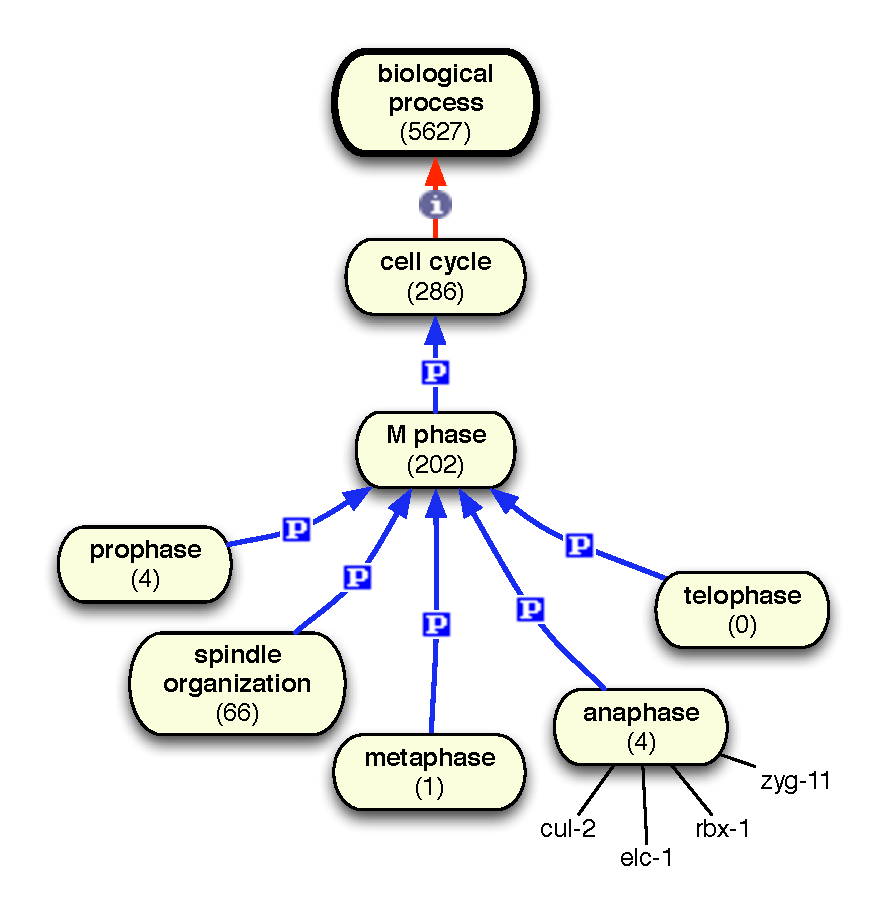
\includegraphics[height=4cm]{dag}
\caption{A view of the Gene Ontology as a Directed Acyclic
  Graph. \emph{SubClassOf} axioms depicted with [i], \emph{SubClassOf
    partOf some} axioms with [p]. Genes for the biological process of
  ``anaphase'' shown. Adapted from\cite{washington2008ontologies}. }
\end{figure}
%----------------------------------------


The users of the GO apply it in a number of ways. The simplest way is
to interrogate a database, for example to find the set of descriptors
for a gene, or to find the set of genes for a descriptor (making use
of the edges in $E$). One of the most common uses is to find a
functional interpretation of a set of genes, a so-called enrichment
test. For example, given a set of genes that become active as a result
of an organism being exposed to an environmental toxin[REF]. Another
use is as a component of a diagnostic tool for finding causative genes
in rare diseases\cite{Phevor}. As of today, the GO has been cited NNN
times (and this is an under-representation of the true use), with XXX
tools dedicated to using the GO, integrated into MMM databases.

This simple formulation of the GO is popular, but outdated, as the GO
has incorporated an ever increasing number of OWL constructs over the
years. The core ontology graph $G$ maps to \emph{SubClassOf} axioms --
either between two named classes (so called is\_a links) or between a
class an expression of the form \emph{R some Y}. Behind the scenes
there are additional axioms, some of which we will describe in this
manuscript.

% ========================================
\section{The Axiomatic Structure and Logic of the GO}
% ========================================

The GO consists of over 40,000 classes, but also includes an import
chain that brings in an additional nnn classes from 6 additional
ontologies. The majority of the axioms in this import chain are within
the EL++ profile, allowing for the use of faster reasoners (we will
describe the small number of axioms outset this profile further on).

The breakdown of axiom types and expression types is as follows
[TABLE]. As can be seen, the most common expression types in GO are
existential restrictions and intersections, with the latter used
almost entirely within equivalence axioms.

The part of GO that is most typically exposed to users are the
SubClassOf axioms (together with annotation assertions), which is weak
in terms of expressivity but delivers the qery abilities required by
most users.

The entire ontology reasons in nn s in Elk\cite{kazakov2012elk}, and nn
minutes in Hermit.

% ----------------------------------------
\subsection{Equivalence axioms in GO}
% ----------------------------------------

The meat and potatoes for reasoning in GO are the equivalence axioms,
most typically of a ``genus-differentia'' form, i.e. \emph{X
  EquivalentTo G and R1 some Y1 and … Rn some Yn}. These were
historically referred to in GO as ‘cross
products’\cite{Mungall2010GOXP}, since the set of such defined classes
$X$ are a subset of the cross-product of the set $G$ and the sets
$Y1..Yn$.

The existence of these axioms allow us to use reasoners to
automatically classify the GO, something that is vitally important in
an ontology with such a large number of classes. This was previously
done entirely by hand, which was time-consuming and error-prone. We
aim to follow the ``Rector Normalization''
pattern\cite{rector_modularisation_2003} as closely as possible but in
practice this is hard, as we are still in the midst of refactoring a
large hand-crafted graph with multiple built-in hidden assumptions. As
this is a labor-intensive procedure, we sometimes break this down into
chunks depending on the external ontology used for normalization. See
for example \cite{Hill2013} which describes refacoring and reasoning
using the CHEBI ontology of chemical entities. Ongoing work involves
the cell type ontology, Uberon and classifications of proteins.

% ----------------------------------------
\subsection{Inter-ontology axioms}
% ----------------------------------------

The subset of GO most commonly exposed comprises the so-called
``intra-ontology'' axioms, but GO also contains a rich set of
inter-ontology axioms. The primary use case for the inter-ontology
axioms is to allow for Rector Normalization and creation of the
inferred hierarchy in GO, but inter-ontology axioms have the added
benefit of connecting different ontologies used for classification of
different types of data.

The version of GO that contains the inter-ontology axioms is called
``go-plus''.

% ----------------------------------------
\subsection{Relations in the GO}
% ----------------------------------------

We use a number of different Object Properties in these axioms, taken
from the OBO Relations
Ontology\footnote{http://code.google.com/p/obo-relations}. The most
commonly used characteristic is Transitivity, and \emph{SubPropertyOf}
and we rely extensively on \emph{SubPropertyChain}.

The majority of relations in RO have an Inverse declared. Typically
within the GO we only use one form, and we never use the
\emph{Inverse} construct in a property expression. One exception to
this is the use of \emph{partOf} and \emph{hasPart}. We frequently
create axioms with an existential restriction using partOf (this forms
the core partonomy of the GO), but have more recently started creating
hasPart axioms\cite{berardini2010gene}. This takes us outside the
profile covered by Elk. However, we are not reliant on the inverse
axiom connecting these two properties for classification purposes. We
have on occasion used this inverse axiom in combination with HermiT to
successfully detect unsatisfiable classes.

% ----------------------------------------
\subsection{Constraints in the GO}
% ----------------------------------------

As well as automatic classification, there is a need for automated
quality control processes. The GO has a large QC pipeline, a subset of
which we implemented via standard OWL reasoning operating over the
axioms in GO.

We encode the majority of constraints in GO as disjointness axioms;
most of the relations used in GO are general and lack specific domain
and range constraints. We achieve more powerful ‘contextual’
domain-range type assertions using disjointness axioms. For example,
the `part of' relation is flexible regarding whether is it used
between processes (for example, a GO biological process such as
‘flower development’) or between ‘static’ material entities (for
example, a GO subcellular component, such as ‘synapse’). This
generality limits the utility of domain and range. However, the RO
includes axioms of the form: `part of' process DisjointWith `part of'
some continuant Which prohibits category-crossing uses of `part of'
which would be invalid.

Disjointness axioms are also used in the traditional way, between
siblings in a taxonomic classification.

We frequently have need to encode spatial and temporospatial
constraints. For example, most of the cells in a complex organism such
as yourself consist of a number of compartments, including the nucleus
(the central HQ, where most of your genes live) and the cytosol (a
kind of soup full of molecular machines doing their business). It’s
not enough to simply state that the cell and cytosol are disjoint
classes. We also want to encode what in RCC8 termiology is the
``disconnected'' relation, the fact that there are no shared parts
(made impossible by the existence of a membrane barrier between the
two). We do this using General Class Inclusion axioms (GCI axioms),
e.g.  

\begin{verbatim}
(`part of' cytosol) DisjointWith (`part of' nucleus)
\end{verbatim}


Another common type of contsraint in the GO are so-called `taxon
constraints' \cite{Deegan2010}. The basic idea here is that the GO
covers biology for all domains of life, from single-celled organisms
to humans. However, many of the classes are applicable to specific
lineages. For example, in describing the function of genes in
Dictyostelium discoideum (slime mold), it would be a mistake to use
the GO class ‘brain development’, as these ameoboid organisms lack a
nervous system of any type. Whilst a human curator would be unlikely
to make such a gross error, the same cannot be said for algorithmic
prediction methods that make use of the `ortholog conjecture' to infer
the function of a gene in one species based on the function of the
equivalent gene in another species. Here it is useful to have a
knowledge-based approach to validation.

Constraints are also used to check the contents of databases. For
example….. TODO

% ----------------------------------------
\subsection{Smuggling OWL expressions into Databases}
% ----------------------------------------


\cite{Huntley2014}

% ----------------------------------------
\subsection{Annotation axioms}
% ----------------------------------------

In addition to the logic axioms described above, GO makes heavy use of
annotation assertion axioms, as the textual component of GO is
important to our users. In particular, textual definitions, comments
and synonyms (in addition to labels) are the annotation properties we
use most commonly.

One of main factors that allowed us to move to OWL was the
introduction of axiom annotations. We attempt to track provenance on a
per-axiom level, so this feature is vital to us.

% ========================================
\section{The GO Development environment}
% ========================================

% ----------------------------------------
\subsection{Editing tools}
% ----------------------------------------

The GO development environment is a hybrid of different tools and
technologies.

In the past, the GO developers exclusively used
OBO-Edit (OE)\cite{Day-Richter2007} for construction and maintenance of the
ontology. OBO-Edit only supports a subset of OBO-Format, which
corresponds roughly to EL++, with the addition of other restrictions,
such as limited ability to nest class expressions. However, the main
limitation of OBO-Edit is the lack of integration with OWL Reasoners
such as Elk (OBO-Edit has a built in rule based reasoner which is too
slow for practical work).

From a formal ontologist perspective, the natural progression is to
switch to editing in Protege. However, whereas Protege excels in areas
such as reasoning and logical axiom editing, it lacks much of the
functionality that makes OBO-Edit a productive and intuitive tool for
the GO developers. These features include powerful search and
rendering, visualization, inclusion of existential restrictions in
hierarchical browsing, as well as annotation editing.

To overcome this we have been moving to a hybrid editing environment,
whereby developers use a mixture of OBO-Edit and Protege. The source
ontology remains in OBO-Format, with the developers using
OWLTools\cite{OWLTools} to perform the conversion to OWL and
back. Developers are careful to remain within the OBO subset of OWL.

At first we employed this hybrid strategy tentatively, with the
developers using Protege primarily as a debugging tool (for example,
explanation of inferences leading to unsatisfiable classes). However,
developers are gradually embracing Protege for other parts of the
ontology development cycle, such as full-blown editing.

To facilitate this transition, we have been collaborating with other
software developers to create plugins that emulate certain aspects of
the OE experience. These include an oboeditor annotation viewer and
editor\footnote{https://github.com/hdietze/protege-obo-plugins}, an
plugin that manages the obsoletion of classes according to GO
lifecycle policy\footnote{https://github.com/balhoff/obo-actions/downloads}, and a partial
port of the OE graph
viewer\footnote{https://code.google.com/p/obographview/}, shown in figure
\ref{fig:gv}.

% ----------------------------------------
\subsection{Web based term submission}
% ----------------------------------------

We have developed a web

TermGenie\cite{Dietze2014}
OWLTools and Oort

% ----------------------------------------
\subsection{Ontology build pipeline}
% ----------------------------------------

Continuous Integration\cite{Mungall2012a}
VCSs and continued use of OBO

TODO: Discussion of obstacles, what we need, when do we want it. Inferring
subclass of 'part of' some Y. More OE like experience in Protege. More
tooling. Something like Maven for ontologies, especially with
dependency/version management.

Currently we have a requirement that ontology developers can switch between use of obo-edit and Protege. Unfortunately, the reasoning support in obo-edit is poor (not integrated with Elk or any standard OWL reasoner). This means that there is effectively no ‘inferred class view’, so we cannot rely on dynamic classification if developers wish to see a rich and complete hierarchy. As a workaround, we have a batch process that mass asserts all direct inferred subclass axioms (and tags these as being asserted via an axiom annotation). In theory these can be deleted and recreated en-masse. In practice this is frankly a rube goldbergesque system that has evolved ad-hoc over the years, and we are planning to overhaul this.

Mention that GO development is closely coordinated with others like CL, UBERON, both in terms of ontology integration and shared infrastructure…

Limitations of MIREOT. We have to mention OBO Foundry efforts here even though in many ways it’s ceased to be of relevance...

Downstream use of the GO. More OWLishness required!

The detailed OWL axiomatization of GO is primarily used within the GO consortium, as a tool for automation and QC during the ontology development lifecycle, and as a database QC tool. However, these more advanced axioms are still not widely used by the many groups developing software the embed or leverage the GO.

Discussion on why this is and what’s to be done…. better integration of statistical/probablistic views and logical….


% ========================================
\section{What does the future hold?}
% ========================================

https://github.com/phenoscape/owlet

GO was designed to be used with a simple database structure, pairwise associations between nodes in the GO graph and molecular entities. 

Where we’re going now: describing complex interactions. How should this be done? ABox or TBox or some mix? 

FIGURE: Noctua

% ========================================
\section{Conclusions}
% ========================================


OWL is great but we want better support, easier tools, ….

A small amount of constructs go a long way: EquivalentClasses, SomeValuesFrom, DisjointWith, SubProperty{Chain}Of
Elk was a game-changer
In many aspects GO axiomatization is of a similar expressivity to earlier DL ontologies like GRAIL. Lessons? Takes a long time for tools to harden, specs to mature and technology to percolate
Foundations of OWL2 are solid (specifications, core APIs) but we need more tools that can be used as part of the ontology development lifecycle. Examples are things like owlet.
How can we get OWL axioms to be used more downstream of the ontology development lifecycle? Should they be? Is the future in integration between DLs and the kinds of statistics and probabilistic reasoning more common in bioinformatics






















% mention stress-testing with OWLAPI

% ========================================
\section{Conclusions}
% ========================================

YADDA

% ========================================
\bibliography{go-owled-paper}
\bibliographystyle{plain}
% ========================================


\end{document}
